%
\chapter{提案手法}
%
\section{モデル概観}
この章では,提案モデルがもつ複合特徴量生成器とニュース分類器について紹介する.
その後にこの2要素を統合して転移学習が可能な表現を学習する方法について説明する.
% 最後に,詳細なアルゴリズムフローを付加する. 
今回提案したモデルは,以下の図\ref{fig:model}の通りとなっている.

提案モデルの目的は,画像とテキストで発信された情報に対して,
正しいニュースか・フェイクニュースか・ジョークニュースかを分類するために,
必要な特徴表現を学習することである.
提案モデルは複合特徴量生成器とニュース分類器の大きく2部分に分けることができる.
まず複合特徴量生成器は,今回扱う情報がテキストと画像を含むため,
各メディアに対して特徴化する生成器がある.
その後それぞれの特徴を1つに連結し,複合特徴となる.
複合特徴はニュース分類器に送られ,最終的には3カテゴリのどれに該当するかが判断される.
% 
\begin{figure}[h]
    \centering
    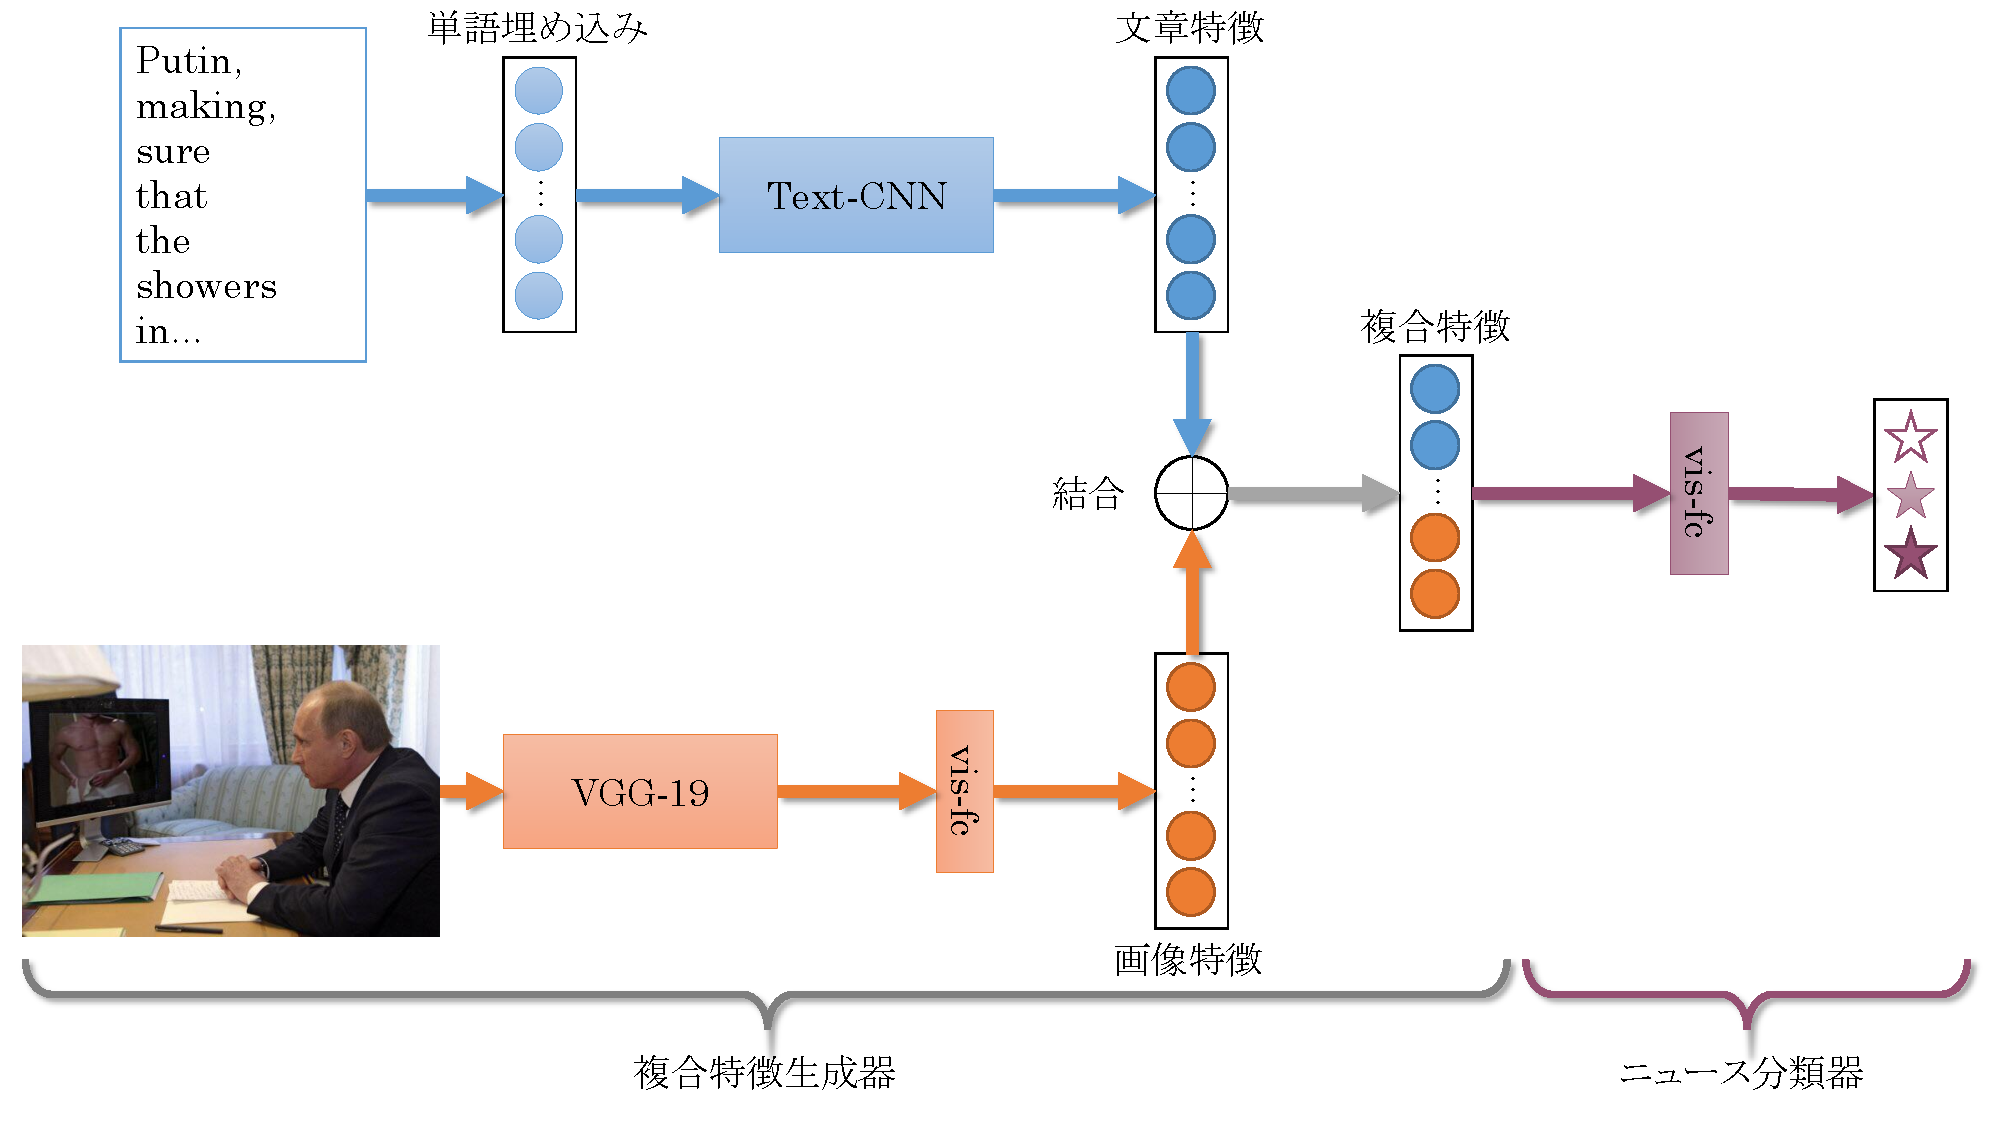
\includegraphics[width=\linewidth]{images/methodology.pdf}
    \caption{提案モデル図.青色がテキスト特徴量生成器,橙色が画像特徴生成器,紫色がニュース分類器である.}
    \label{fig:model}
\end{figure}

%
\section{複合特徴生成器}
%

%
\section{ニュース分類器}
%


%図の挿入


%
%
\newpage
%
%
%
%
%
%
%
%
%
%
% 